%; whizzy section -pdf xpdf -latex ./whizzypdfptex.sh
% latex beamer presentation.
% platex, latex-beamer でコンパイルすることを想定。 

%     Tokyo Debian Meeting resources
%     Copyright (C) 2007 Junichi Uekawa

%     This program is free software; you can redistribute it and/or modify
%     it under the terms of the GNU General Public License as published by
%     the Free Software Foundation; either version 2 of the License, or
%     (at your option) any later version.

%     This program is distributed in the hope that it will be useful,
%     but WITHOUT ANY WARRANTY; without even the implied warranty of
%     MERCHANTABILITY or FITNESS FOR A PARTICULAR PURPOSE.  See the
%     GNU General Public License for more details.

%     You should have received a copy of the GNU General Public License
%     along with this program; if not, write to the Free Software
%     Foundation, Inc., 51 Franklin St, Fifth Floor, Boston, MA  02110-1301 USA

% 実行順番
% sudo  ~/bin/usb-macbook-ir.c &
% real presentation (shell-command (concat "DISPLAY=:0.1 xpdf -fullscreen " (replace-regexp-in-string "tex$" "pdf"(buffer-file-name)) "&"))
% DISPLAY=:0.1 xpdf -fullscreen 

\documentclass[cjk,dvipdfmx,12pt]{beamer}
\usetheme{Tokyo}
\usepackage{ulem}
\usepackage{tabularx}


%  preview (shell-command (concat "evince " (replace-regexp-in-string "tex$" "pdf"(buffer-file-name)) "&"))
%  presentation (shell-command (concat "xpdf -fullscreen " (replace-regexp-in-string "tex$" "pdf"(buffer-file-name)) "&"))

%http://www.naney.org/diki/dk/hyperref.html
%日本語EUC系環境の時
\AtBeginDvi{\special{pdf:tounicode EUC-UCS2}}
%シフトJIS系環境の時
%\AtBeginDvi{\special{pdf:tounicode 90ms-RKSJ-UCS2}}

\title{東京エリア Debian 勉強会}
\subtitle{資料}
\author{上川 純一 dancer@debian.org\\IRC nick: dancerj}
\date{2007年7月21日}
\logo{
\includegraphics[width=8cm]{image200607/openlogo-light.eps}}


% 間のタイトルページ用
\newcommand{\emtext}[1]{
\begin{frame}{}
 
\begin{minipage}{0.55\hsize}
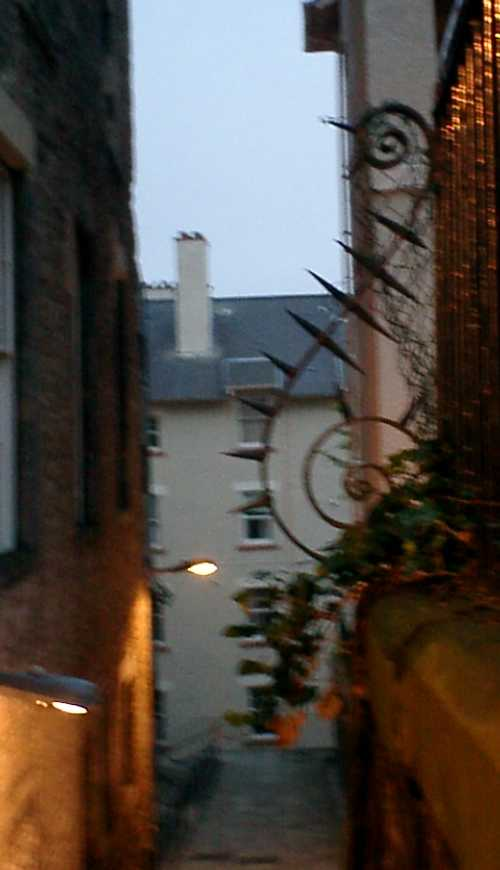
\includegraphics[width=1\hsize]{image200707/gurutitle.jpg}
\end{minipage}
\begin{minipage}{0.39\hsize}
 {\Huge #1
 }
\end{minipage}
\end{frame}
}

% 三択問題用
\newcounter{santakucounter}
\newcommand{\santaku}[5]{%
\addtocounter{santakucounter}{1}
\frame{\frametitle{問題\arabic{santakucounter}. #1}
%問題\arabic{santakucounter}. #1
\begin{minipage}[t]{0.8\hsize}
 \begin{itemize}
 \item
      \begin{minipage}{0.2\hsize}
      
\includegraphics[width=0.9\hsize]{image200703/janken-A.png}\end{minipage} 
       \begin{minipage}{0.6\hsize}
       A #2\end{minipage}\\
 \item
      \begin{minipage}{0.2\hsize}
      
\includegraphics[width=0.9\hsize]{image200703/janken-B.png}\end{minipage} 
       \begin{minipage}{0.6\hsize}
       B #3\end{minipage}\\
 \item
      \begin{minipage}{0.2\hsize}
      
\includegraphics[width=0.9\hsize]{image200703/janken-C.png}\end{minipage} 
       \begin{minipage}{0.6\hsize}
       C #4\end{minipage}\\
 \end{itemize}
\end{minipage}
}
\frame{\frametitle{問題\arabic{santakucounter}. #1}
%問題\arabic{santakucounter}. #1
\begin{minipage}[t]{0.8\hsize}
\begin{itemize}
 \item
      \begin{minipage}{0.2\hsize}
      
\includegraphics[width=0.9\hsize]{image200703/janken-A.png}\end{minipage} 
       \begin{minipage}{0.6\hsize}
       A #2\end{minipage}\\
 \item
      \begin{minipage}{0.2\hsize}
      
\includegraphics[width=0.9\hsize]{image200703/janken-B.png}\end{minipage} 
       \begin{minipage}{0.6\hsize}
       B #3\end{minipage}\\
 \item
      \begin{minipage}{0.2\hsize}
      
\includegraphics[width=0.9\hsize]{image200703/janken-C.png}\end{minipage} 
       \begin{minipage}{0.6\hsize}
       C #4\end{minipage}\\
\end{itemize}
\end{minipage}
\begin{minipage}[t]{0.15\hsize}
答えは:

\vspace{1cm}

  {\huge \hspace{1cm}#5}
  \hspace{-6cm}\includegraphics[width=4cm]{image200703/janken-#5.png}
 \end{minipage}}
}

\begin{document}
\frame{\titlepage{}}

\section{Intro}

\begin{frame}
 \frametitle{本日のagenda}
\begin{minipage}[t]{0.45\hsize}
  \begin{itemize}
  \item 注意事項
	\begin{itemize}
	 \item 飲食禁止
	 \item 政治/宗教/営利活動禁止
	\end{itemize}
  \item quiz
  \item Debconf7 報告
	\begin{itemize}
	 \item 概要
	 \item 議論
	\end{itemize}
 \end{itemize}
\end{minipage} 
\begin{minipage}[t]{0.45\hsize}
 \begin{itemize}
  \item Debconf workshop
	\begin{itemize}
	 \item 事前課題検討
	 \item Debconf で得るもの
	 \item Debconf を日本で開催するには
	\end{itemize}  
\item Debian 勉強会の今後の企画の検討
 \end{itemize}
\end{minipage}
\end{frame}

\section{最近}

\begin{frame}
 \frametitle{前回のagenda}
\begin{minipage}[t]{0.45\hsize}
  \begin{itemize}
  \item 注意事項
	\begin{itemize}
	 \item 飲食禁止
	 \item 政治/宗教/営利活動禁止
	\end{itemize}
  \item quiz
  \item Debconf7 リハーサル
	\begin{itemize}
	 \item pbuilder 
	 \item superh
	\end{itemize}
 \end{itemize}
\end{minipage} 
\begin{minipage}[t]{0.45\hsize}
 \begin{itemize}
  \item エッチ
	\begin{itemize}
	 \item サーバをエッチにしてみました
	 \item 事前課題紹介
	 \item エッチワークショップ
	\end{itemize}  
\item Debian 勉強会の今後の企画の検討
 \end{itemize}
\end{minipage}
\end{frame}

\section{DWN quiz}
\begin{frame}{Debian 常識クイズ}

Debian の常識、もちろん知ってますよね?
しらないとはずかしいけどしらないとは言えないいろいろなこと、
Debian Weekly News をベースに確認してみましょう。

\end{frame}

\subsection{2007年6号}
\url{http://www.debian.org/News/weekly/2007/06/}
にある7月3日版です。

\santaku
{Andr\'e Luiz Rodrigues Ferreira が宣言したのはどのウェブサイトか}
{Debian art}
{Debian pop}
{Debian tart}
{A}

\santaku
{J\"ulich で行われた会議で lenny のリリースプロセスについて何をすることが決まったか}
{秘密のプロセスにのっとり、今後リリースがどうなっているかは非公開にする}
{毎月か二ヶ月に一回の最終週にリリース状況についてのメールを出す}
{安全保障のため今後は Debian Developerでないとリリースの状況がわからないようにする}
{B}

\santaku
{Lucas Nussbaum は毎月何をすると発表したか}
{深刻な問題のあるパッケージを順番にのっとる}
{深刻な問題のあるパッケージを管理している人に罰ゲームをさせる}
{深刻な問題のあるパッケージについて通知するメールを自動で送付}
{C}

\santaku
{Alexander Wirt は何を発表したか}
{backports.org が sid に対応}
{backports.org が lenny に対応}
{backports.org が etch に対応}
{C}

\santaku
{Martin Michlmyr が挑戦しているのは何か}
{Debian を gcc 4.2でビルドできるようにする}
{Debian を全部 C++ におきかえる}
{Debian を全部 ruby におきかえる}
{A}


\section{Debconf7 agenda}

\emtext{Debconf7紹介}

\begin{frame}
 \frametitle{Debconf7紹介 agenda}
\begin{minipage}[t]{0.45\hsize}
  \begin{itemize}
  \item Debconf7 紹介
	\begin{itemize}
	 \item 歴史
	 \item 会場
	 \item メンバー
	\end{itemize}
 \end{itemize}
\end{minipage} 
\begin{minipage}[t]{0.45\hsize}
 \begin{itemize}
  \item 討議内容
	\begin{itemize}
	 \item 組込み ARM EABI, Emdebian, Superh
	 \item i18n
	 \item 品質管理
	\end{itemize}  
  \item Q\&A
 \end{itemize}
\end{minipage}
\end{frame}

\emtext{Debconf7紹介}

\section{Debconf7 紹介}
\begin{frame}{歴史}
Debian Project の開発者をあつめて技術的な内容を討議する年次のカンファレンス
 \begin{tabular}{|c|c|c|r|}
 \hline
 年 & 名前 & 場所 & 参加人数 \\
 \hline
 2000 & debconf 0 &フランス ボルドー & \\
 2001 & debconf 1 &フランス ボルドー & \\
 2002 & debconf 2 &カナダ トロント & 90名 \\
 2003 & debconf 3 &ノルウェー オスロ & 140名 \\
 2004 & debconf 4 &ブラジル ポルトアレグレ &  150名 \\
 2005 & debconf 5 &フィンランド ヘルシンキ & 200名 \\
 2006 & debconf 6 &メキシコ オアスタペック & 300名 \\
 2007 & debconf 7 &スコットランド エジンバラ & 400名 \\
 2008 & debconf 8 &アルゼンチン マルデプラタ & ?名 \\
 \hline
 \end{tabular}
\end{frame}

\begin{frame}{会場 1/2}
\begin{minipage}{0.49\hsize}
 会場は昼の会場(Teviot)と夜の会場(廃教会)にわかれた。

  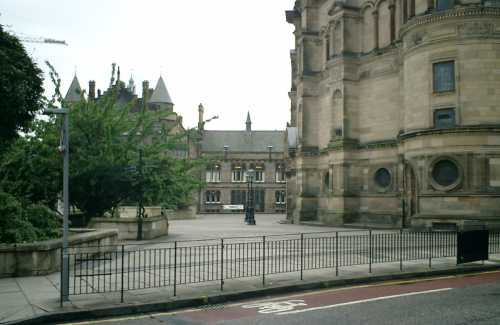
\includegraphics[width=1\hsize]{image200707/teviot.jpg}
\end{minipage}
\begin{minipage}{0.49\hsize}
  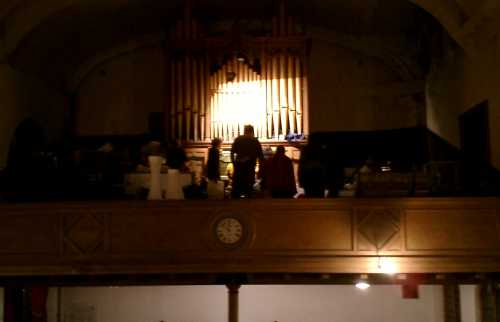
\includegraphics[width=1\hsize]{image200707/nightvenue1.jpg}\\
  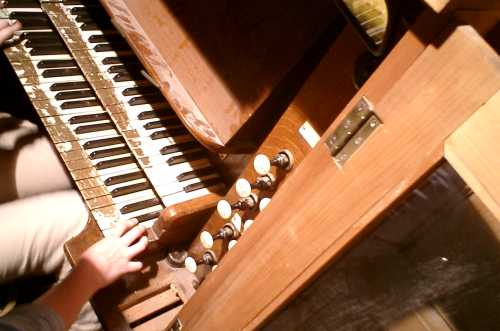
\includegraphics[width=1\hsize]{image200707/nightvenue2.jpg}
\end{minipage}
\end{frame}

\begin{frame}{会場 2/2}
\begin{minipage}{0.49\hsize}
  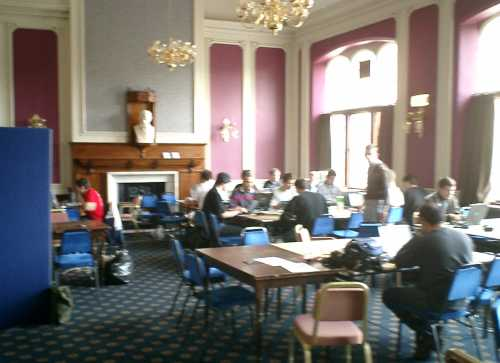
\includegraphics[width=1\hsize]{image200707/hacklab.jpg}\\
  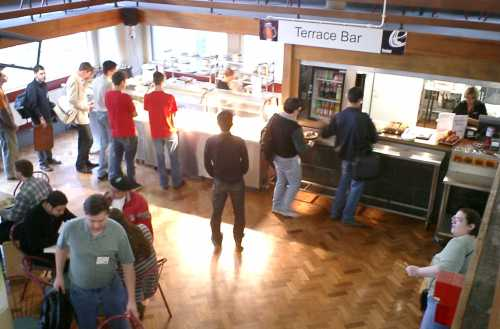
\includegraphics[width=1\hsize]{image200707/lunchplace.jpg}
\end{minipage}
\begin{minipage}{0.49\hsize}
  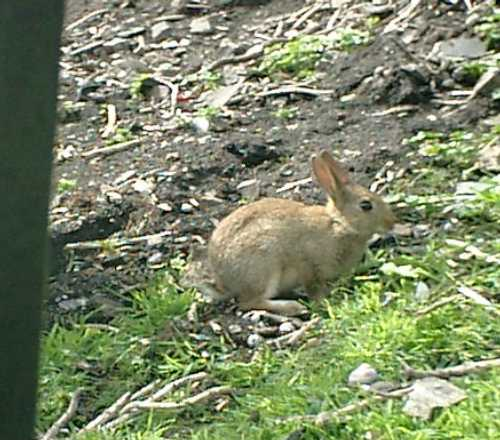
\includegraphics[width=1\hsize]{image200707/rabbit.jpg}\\
  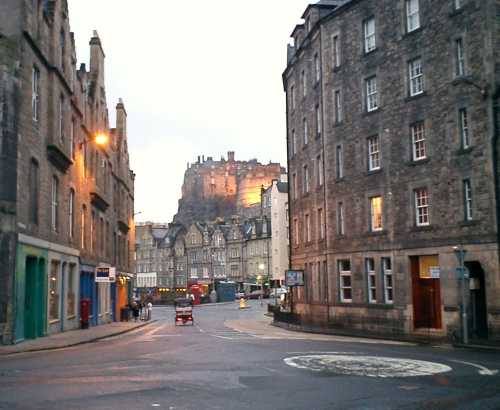
\includegraphics[width=1\hsize]{image200707/castle.jpg}
\end{minipage}
\end{frame}

\begin{frame}{アジェンダ 1/2}
  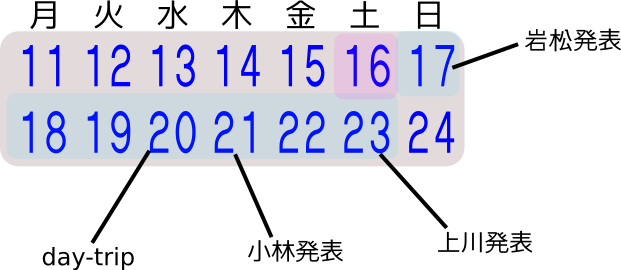
\includegraphics[width=1\hsize]{image200707/schedule.png}\\
発表内容:\\
岩松: superh 移植版について\\
小林: i18n関連\\
上川: pbuilder, cowbuilder, qemubuilder
\end{frame}

\begin{frame}{アジェンダ 2/2}
  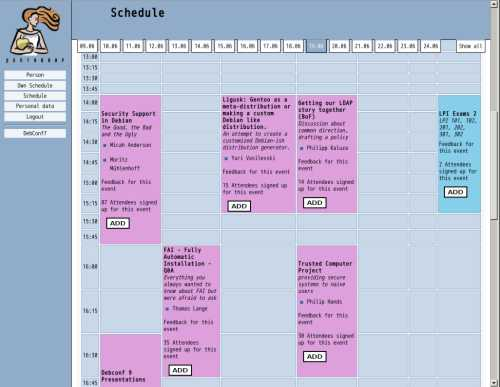
\includegraphics[height=0.6\vsize]{image200707/penta.png}\\
 スケジュールは pentabarf システムで管理、随時変更がかかる

 IRC チャンネルで IRC bot が開催が近くなると通知
\end{frame}

\begin{frame}{参加メンバー}
 2007年は日本からは岩松、矢吹、上川が参加

  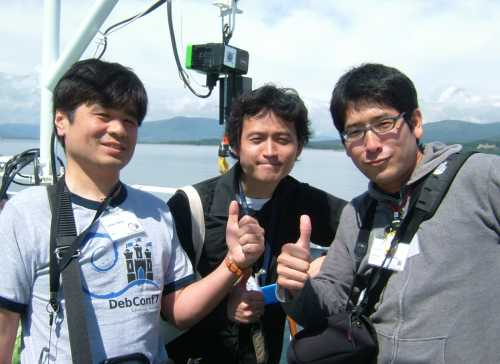
\includegraphics[width=1\hsize]{image200707/members.jpg}
\end{frame}

\begin{frame}{day-trip}
\begin{minipage}{0.5\hsize}
Bute 島への一日旅行

コンピュータに全く触れない一日をスケジュールの真ん中に準備することで長い
 会期をのりきる

新しいインスピレーションがうまれたり

新しいコミュニケーションができたり
\end{minipage}
\begin{minipage}{0.48\hsize}
  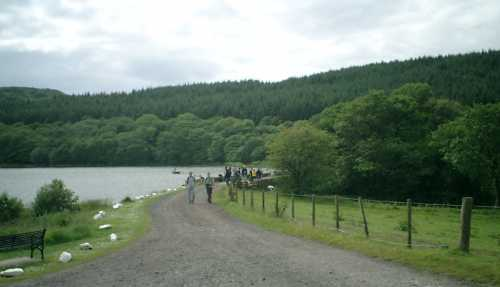
\includegraphics[width=1\hsize]{image200707/daytrip1.jpg}\\
  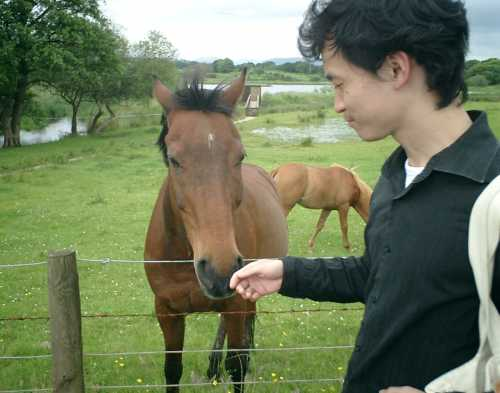
\includegraphics[width=1\hsize]{image200707/daytrip2.jpg}
\end{minipage}
\end{frame}

\emtext{討議内容}

\section{組込 関係の話題}
\begin{frame}
\frametitle{組込 関係の話題}
\begin{itemize}
\item Armel port
\item Emdebian
\item SuperH
\end{itemize}
\end{frame}

\section{Armel port}
\begin{frame}
\frametitle{Armel port} 
  \begin{minipage}{0.45\hsize}
    \begin{itemize}
      \item 発表者

	Wooky
    \end{itemize}
  \end{minipage}
  \begin{minipage}{0.45\hsize}
    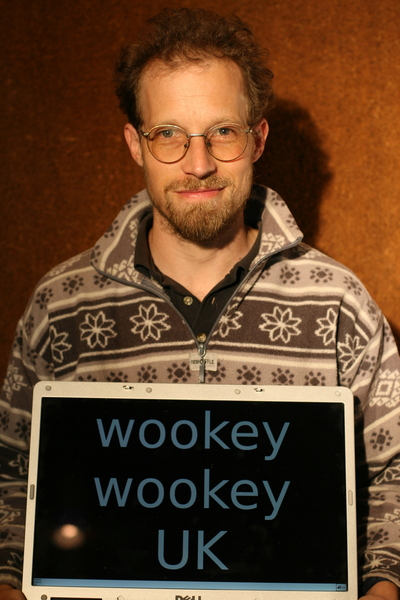
\includegraphics[width=4cm]{image200707/wookey.jpg}
  \end{minipage}

\end{frame}

\begin{frame}
\frametitle{Armelとは} 
\begin{itemize}
  \item Armel

     ARM への新しい ポーティング名 

  \item 二種類の ABI
    \begin{itemize}
	\item legacy ABI

	  従来の ABI
        \item ARM EABI

	  組込向けの ABI 
    \end{itemize}
\end{itemize}
\end{frame}

\begin{frame} 
\begin{itemize}
  \item legacy ABI
    \begin{itemize}
     
	\item FPU 命令コードの取扱い
	\item 例外による浮動小数点演算
    \end{itemize}

  \item EABI
    \begin{itemize}
	\item 動的な FPU を使った計算とソフトウェアによる計算
    \end{itemize}
\end{itemize}
  この2つに互換性はない
\end{frame}


\begin{frame}
\frametitle{現在の状況} 
\begin{itemize}
  \item binutils

	2.16.92 からサポート
  \item gcc
	
	gcc-4.1.1 からサポート
  \item glibc
	
	glibc-2.4 からサポート
  \item linux-kernel

	2.6.16 からサポート
  \item Debian packages

	現在、約10000パッケージをサポート
\end{itemize}
\end{frame}


\begin{frame}
\frametitle{今後の課題} 
\begin{itemize}
  \item 旧バイナリから新バイナリへの移行

	debtakeover\footnote{他のLinuxディストリからDebianに移行するための補助ツール} 
	を使うことによって、移行が容易になるはず。
 

\end{itemize}
\end{frame}


\section{Emdebian}
\begin{frame}
\frametitle{発表者} 
  \begin{minipage}{0.3\hsize}
    \begin{itemize}
      \item 発表者

	Wooky

        Neil Williams
    \end{itemize}
  \end{minipage}
  \begin{minipage}{0.6\hsize}
    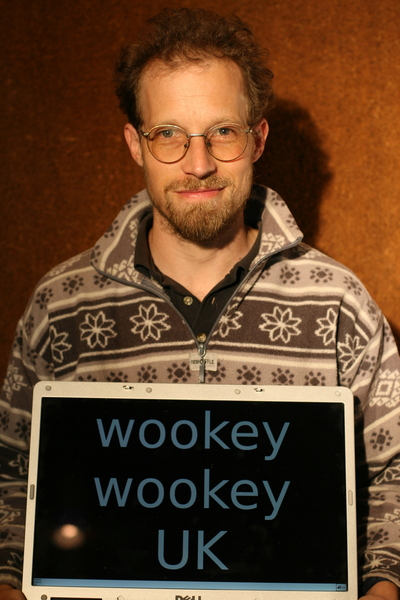
\includegraphics[width=4cm]{image200707/wookey.jpg}
    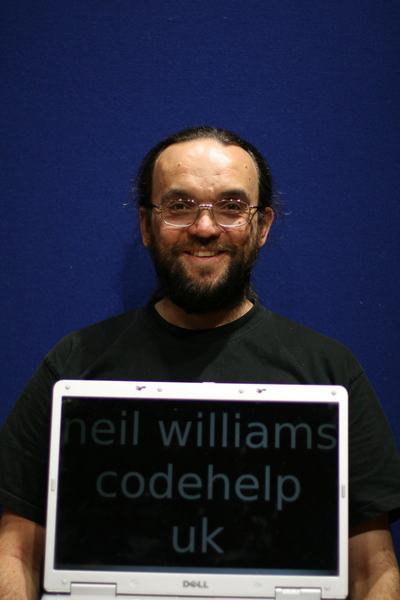
\includegraphics[width=4cm]{image200707/codehelp.jpg}  
  \end{minipage}

\end{frame}

\begin{frame} 
\frametitle{Emdebian}
  \begin{itemize}
    \item 2000 年から開始.
    \item Debian の組込向け プロジェクト
    \item 正式なサブプロジェクトのひとつ
    \item クロスコンパイルによるパッケージのサポート 
  \end{itemize}
\end{frame}

\begin{frame} 
\frametitle{いままで試してきたことについて}
  \begin{itemize}
    \item Debian は native コンパイル思考

	→ クロスコンパイルをサポートするように、パッケージにサポート修正

    \item Debian は パッケージサイズが大きく、デスクトップ思考
	
	→ パッケージを作成するときにドキュメントを外す仕組みを追加

    \item ソフトウェア毎に最適化する仕組み

    \item glibc 以外の C library を試用

    \item perl に頼らない Debian system の構築

	→ Essential から Perl package を外す
  \end{itemize}
\end{frame}


\begin{frame} 
\frametitle{現在のステータス}
  \begin{itemize}
    \item dpkg, apt, debhelper に cross 用のツールを追加
    \item cross 用のツールを用意

	\begin{itemize}
		\item dpkg-cross
		\item apt-cross
		\item emdebian-tools
		  %debuild → emdebuild
		  %dh_make → em_make
	\end{itemize}
    \item ドキュメント類を削除したパッケージを用意
    \item emdebian の changelog, patch を subversion で管理
    \item i386/ppc/amd64 用のクロスコンパイル環境の提供 
  \end{itemize}
\end{frame}


\begin{frame} 
\frametitle{解決すべき問題点など}
  \begin{itemize}
    \item configure のクロスコンパイル対応

	configure 実行するときに --host, --target を指定していないものが多い

    \item configure のドキュメント対応

	-nodocs, -nocheck に対応していない configure が多い

    \item テストプログラム

	コンパイル途中で動作するテストプログラムを実行しないで済む仕組みが
	必要 
  \end{itemize}
\end{frame}



\begin{frame} 
\frametitle{今後の予定}
  \begin{itemize}
    \item ツールチェイン自動アップデート
    \item GPE for ARM
    \item emdebuild
    \item empdebuild
    \item configure キャッシュファイルのサポート 
  \end{itemize}
\end{frame}


\begin{frame} 
\frametitle{Emdebian BOF}
  \begin{itemize}
    \item uClibc サポートの議論
	\begin{itemize}
	  \item バイナリ非互換
	  \item メンテナンス性、サーバー容量の問題
	\end{itemize}
    \item Busybox サポートの議論
	\begin{itemize}
	  \item GPE が 使用
	  \item busybox 上でのパッケージサポート
	\end{itemize}
  \end{itemize}
\end{frame}


\section{Debian for SuperH}
\begin{frame}
\frametitle{Debian for SuperH} 
  \begin{minipage}{0.4\hsize}
    \begin{itemize}
      \item 発表者

	Nobuhiro Iwamatsu
    \end{itemize}
  \end{minipage}
  \begin{minipage}{0.4\hsize}
    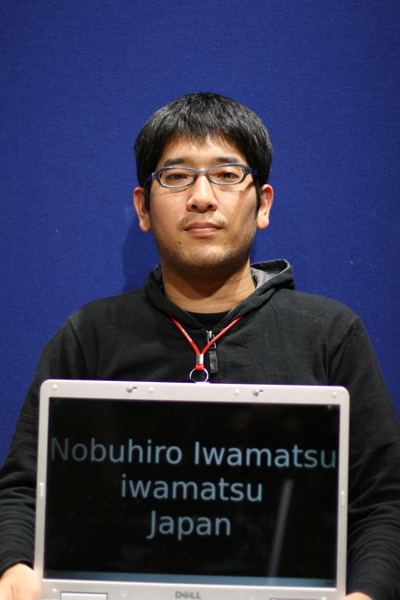
\includegraphics[width=4cm]{image200707/iwamatsu.jpg}  
  \end{minipage}
\end{frame}


\begin{frame} 
\frametitle{今までの移植の歴史}
  \begin{itemize}
    \item 自分が行うまでに2回移植が行われた
    \item しかし、全て失敗
    \item 世界を巻き込んでやらないといけない

	世界の興味ある人を募集中。 
  \end{itemize}
\end{frame}


\begin{frame} 
\frametitle{ポーティングポリシー}
  \begin{itemize}
    \item サポートアーキテクチャ

	SH4 / little

    \item SH3 : FPU / Calling convention / Cache   
    \item Big Endian
	
  \end{itemize}
\end{frame}


\begin{frame} 
\frametitle{現在の状況}
  \begin{itemize}
    \item Maling list
    \item Buildd 動作中   
    \item Build-essential
    \item 2000パッケージビルド
  \end{itemize}
\end{frame}

\begin{frame} 
\frametitle{TODO}
  \begin{itemize}
    \item buildd / アーキテクチャ メンテナンスチーム
    \item SH 特有の問題を解決   
    \item Buildd.net への登録
  \end{itemize}
\end{frame}


\begin{frame} 
\frametitle{現在入手可能な SH デバイス紹介}
  \begin{itemize}
    \item ULS-5P
    \item T-SH7706-LAN   
    \item L-BOX
    \item PX-EH16L
  \end{itemize}
\end{frame}

\begin{frame} 
\frametitle{議論}
  \begin{itemize}
    \item SH4A コアなどの対応
    \item キャッシュ問題の回避方法
    \item マシンの入手の問題
  \end{itemize}
\end{frame}

\section{i18n 関係の話題}

\begin{frame}
\frametitle{i18n 関係の話題} 
Debconf7 で行われた i18n (internationalization) のセッション
  \begin{itemize}
     \item i18n work session
     \item Quality assurance activities for localization    
  \end{itemize}
\end{frame}


\begin{frame}
\frametitle{i18n work session} 
  \begin{minipage}{0.4\hsize}
    \begin{itemize}
      \item 発表者

	Christian Perrier
    \end{itemize}
  \end{minipage}
  \begin{minipage}{0.4\hsize}
    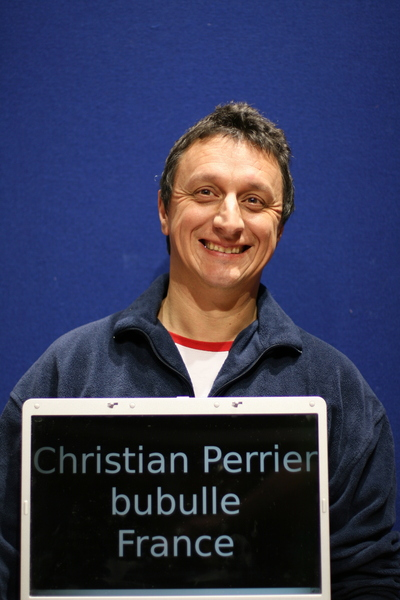
\includegraphics[width=4cm]{image200707/bubulle.jpg}  
  \end{minipage}
\end{frame}

\begin{frame}
\frametitle{i18n work session} 
期間中に8回のセッションが行われた.

  \begin{itemize}
     \item Launch session
     \item Lenny i18n release goals
     \item Pootle session
     \item DDTP, DDTSS, discussion about DDTP import to Pootle
     \item i18n  translation licensing, website, documentation
     \item i18n No content yet..:-)
     \item "tdebs", dpkg/apt, classes of files
     \item Conclusion session    
    
  \end{itemize}
\end{frame}

\begin{frame}
\frametitle{Quality assurance activities for localization} 
  \begin{minipage}{0.4\hsize}
    \begin{itemize}
      \item 発表者

	\sout{Noritada Kobayashi}

        代打 Junichi Uekawa
    \end{itemize}
  \end{minipage}
  \begin{minipage}{0.4\hsize}
    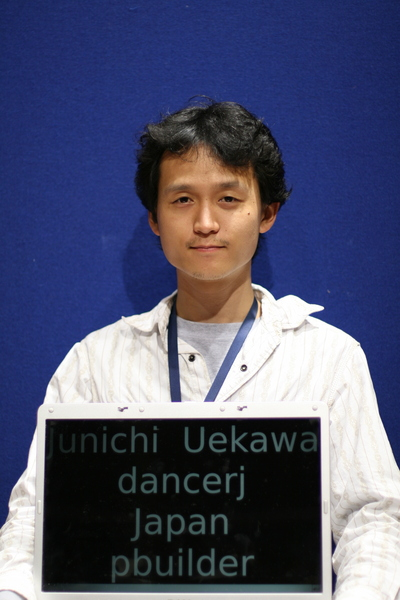
\includegraphics[width=4cm]{image200707/dancerj.jpg}  
  \end{minipage}
\end{frame}


\begin{frame}
\frametitle{セッション内容}

  どのようなツールを使って翻訳を行っているのか.
  \begin{itemize}
    \item pootle

	翻訳向けポータルサイトツール
	\url{i18n.debian.net:8080}
    \item robot

	現在、Debian 翻訳チームが使っているツール
	\url{i18n.debian.net/debian-l10n}\\
    \item 翻訳ツール
	\begin{itemize}
	  \item emacs/vi po-mode
          \item poedit
        \end{itemize}

    \item 翻訳補助ツール
	\begin{itemize}
	   \item kbabel / vi spell check など 
	   \item pootel でも可能
	\end{itemize}

    \item 現在のワークフローや情報

	\url{http://i18n.debian.net/wiki}
  \end{itemize}
\end{frame}


\section{品質管理 関係の話題}
\begin{frame} 
\frametitle{品質管理 関係の話題}

  \begin{itemize}
    \item Proactive Bug Discovery
    \item Maintaining Packages With Git
    \item WTFM, again: Write The Fine Manual page
  \end{itemize}
%Automated Testing of Debian Packages: Status Update
%bugs.debian.org and debbugs
%Debian Documentation Project: current status and future
%Debtags is ready
%Forking Debian every day
\end{frame}



\begin{frame} 
\frametitle{WTFM, again: Write The Fine Manual page}
  \begin{minipage}{0.4\hsize}
    \begin{itemize}
      \item 発表者

	W. Borgert
    \end{itemize}
  \end{minipage}
  \begin{minipage}{0.4\hsize}
    No Photo  
  \end{minipage}
\end{frame}

\begin{frame} 
\frametitle{WTFM, again: Write The Fine Manual page}
  いかにして、品質のよい man page を作成するか.

  \begin{itemize}
    \item Debian で頒布されているプログラムにはマニュアルが必要
    \item nroff 形式の man が多いが時代遅れ

	あらゆるフォーマットに対応できる形式が望ましい
    \item docbok-xml を使うとよい
	
	Gnome, KDE, Linux などで採用
    \item マニュアルがソースに含まれている場合もあるが、チェックが必要
  \end{itemize}	
\end{frame}

\begin{frame} 
\frametitle{Proactive Bug Discovery}
  \begin{minipage}{0.4\hsize}
    \begin{itemize}
      \item 発表者

	Sam Hocevar / Debian Project Leader
    \end{itemize}
  \end{minipage}
  \begin{minipage}{0.4\hsize}
    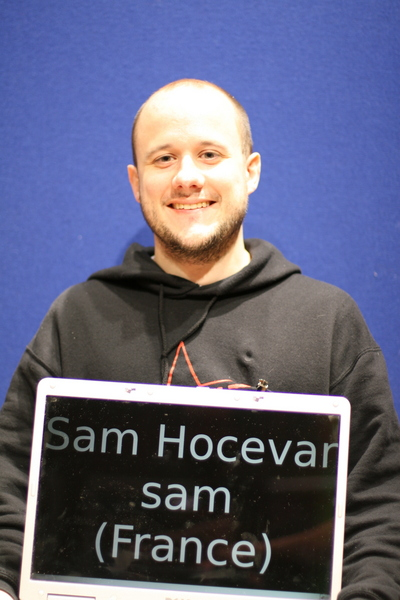
\includegraphics[width=4cm]{image200707/sam.jpg}
  \end{minipage}
\end{frame}

\begin{frame} 
\frametitle{Proactive Bug Discovery}
  パッケージの不具合を見つけるには

  \begin{itemize}
    \item ソースコードから見つける
	\begin{itemize}
	  \item google code search
	  \item rats, pscan, jlint, pychecker
	\end{itemize}

    \item コンパイル時に -Wall をつけよう
    \item makewrap の活用
	
	LD\_PRELOAD=makewrap.so debian/rules
	
    \item build log を参照

	http://buildd.debian.org

  \end{itemize}	
\end{frame}


\begin{frame} 
\frametitle{Proactive Bug Discovery}
  バイナリパッケージから不具合を見つける

  \begin{itemize}
    \item Debian Policy によるチェック
	
	linda / lintian
	
    \item インストール/アンインストールチェック

	piuparts

    \item Fuzzing の活用
	
	zzuf パッケージを使ったテスト方法

    \item GUI アプリケーション のデバッグ
	
	xvfb の活用

    \item test suite の活用

  \end{itemize}	
\end{frame}


\begin{frame} 
\frametitle{Maintaining Packages With Git}
  \begin{minipage}{0.4\hsize}
    \begin{itemize}
      \item 発表者

	David Nusinow
    \end{itemize}
  \end{minipage}
  \begin{minipage}{0.4\hsize}
    no photo
  \end{minipage}
\end{frame}


\begin{frame} 
\frametitle{Maintaining Packages With Git}
  git, git-buildpackage を使って、debian package を管理する方法
	
  \begin{itemize}
    \item X strikeforce は gitを使っている
    \item patch 管理 は quilt を使う
    \item git を使うだけで時間の節約になる
    
	各種ツールがはやい. branch が楽.

    \item svn ではコミットに制限があるが git にはない

	どこでもコミット.

    \item git-xxx

	他の SCM で管理しているアップストリームを git で管理するのに楽

	
  \end{itemize}
\end{frame}


\begin{frame} 
\frametitle{Maintaining Packages With Git}
  git, git-buildpackage を使って、debian package を管理する方法
	
  \begin{itemize}
    \item debcommit
	debian/changelog を各 SCM のコミットメッセージとして扱ってくれるツール

    \item 問題
      \begin{itemize}
	 \item git-buildpackage は
	       アップストリームが git を使っている場合に、うまく動作しない
	 \item git の Windows ネイティブ版が普及していない\footnote{
	       cygwin 版、mingw 版はある }
         \item git ではディレクトリ毎にチェックアウトできない\footnote{submodule
	       機能実装中}
      \end{itemize}
  \end{itemize}
 
\end{frame}


\section{Debconf7 の情報}
\begin{frame} 
\frametitle{Debconf7の情報 }
\begin{itemize}
    \item \url{http://debconf7.debconf.org}
    \item \url{http://wiki.debconf.org/wiki/DebConf7}
  \end{itemize}
\end{frame}

\section{次の Debconf}
\begin{frame} 
\frametitle{次の Debconf }
\begin{center}

\includegraphics[width=10cm]{image200707/debconf8.png}  
 \end{center}  
\begin{itemize}
    \item アルゼンチン
    \item 8月 (開催地は冬です)
  \end{itemize}
\end{frame}

\emtext{Debconf Workshop}

\section{事前課題紹介}
\emtext{事前課題の紹介}

\begin{frame}{事前課題問題}
「今後Debconfを日本で開催するためにDebianの認知度を上げる方法」もしくは
「企業がDebconfのスポンサーになるためには」
というタイトルで200-800文字程度の文章を書いてください。
\end{frame}

\begin{frame}{Hideki Yamane}

\textbf{企業がDebconfのスポンサーになるためには}

これは実際に debconf7 のスポンサーをした企業に聞いてみるのが良いのではないかと。
\url{https://debconf7.debconf.org/wiki/Main_Page} で一覧が見れます。


\end{frame}\begin{frame}{Aya Komuro}


\textbf{今後Debconfを日本で開催するためにDebianの認知度を上げる方法}

\begin{itemize}
 \item  Debianを使っている人のブログにブログシールを貼ってもらう
 \item  Debianの壁紙(PC/携帯など)を作って配布
 \item  日本にあるジオキャッシングのポイントの宝物を全部Debianのインストール
 CD/DVDにしておく
 \item  Debianウチワを作って道行く人に配布
 \item  DebianJP(など)についてを漫画にしてみる
\end{itemize}


\end{frame}\begin{frame}{Kouhei Maeda 1/3}

\textbf{「今後Debconfを日本で開催するためにDebianの認知度を上げる方法」
「企業がDebconfのスポンサーになるためには」}

日本だと、Linuxをちょっと知っている程度の人はLinux=Redhatだと思います。
スポンサーになる決裁権限を持っている人もまた然り。Linux自体知らないかも
しれません。そう考えると、「Debian?何ソレ?」ということになるだろうと。

そうするとDebian自体の認知度を上げる対象としては、Linuxをかろうじて知っているレベルの人、あわよくばLinux自体を知らない一般の人になるかと。

\end{frame}\begin{frame}{Kouhei Maeda 2/3}

\begin{itemize}
 \item  Linuxを知っている人
 \begin{enumerate}
 \item Debianというディストロ自体の存在を教える。
 \item Debianの特徴を話す。
 \item Redhatなど(というかRedhatだけで十分だろうけど)他のディストロと比較したときのメリット、デメリットを説明する。
 \item ビジネスでDebianを使うとき…の話になると、スポンサーやるだけの体力のある会社(そもそもスポンサーは最低いくらから?という疑問があるのですが)で、Debianを導入する企業は、初期費用が高くてRedhatはもちろん、Windows、商用Unixなんぞ使わん!という企業な気がします。そこの(現場でがちがちにやっている人ではなく)決裁権限を持った人を対象にDebianを使いましょうセミナー(OSCとか?)やるんでしょうか…。
 \end{enumerate}
\end{itemize}
\end{frame}\begin{frame}{Kouhei Maeda 3/3}
\begin{itemize}
 \item  Linuxを知らない人
 \begin{enumerate}
 \item Linuxとは何ぞやという話をする。
 \item Linux=Debianというくらいの勢いでDebianの良さを刷り込む。
 \end{enumerate}
 終了。
\end{itemize}

どちらにしても、一般の人を対象にしたDebianの普及活動が必要ではないかなと思います。

とりあえず個人でできることとしては、4月から月一でやっている社内のLinux勉強会では、自分での担当分の資料とか話は全部Debianでやってます。Debianって何?というか、Linux自体使ったことない人もかなり多いので。

\end{frame}\begin{frame}{岩崎 修}

\textbf{今後Debconfを日本で開催するためにDebianの認知度を上げる方法}

とかくDebianというと「難しい」「堅苦しい」というようなステロタイプがあるように思えます、というか私はそう思っていました。

ところが、いろいろとディスリビューションを試したあげく、出た結論は、私のような小規模な会社で各種サーバーを立てる際には、Debianが一番、設定も日常の管理も楽であるということでした。

たまたま、一昨日から「社内のいろんなこと全部させているサーバー(apache,
zope,サイボウズOffice他)」をリプレースするにあたって、etchをインストール
\& 設定しているところなのですが、非常にお気軽にだいたいの作業が済んでしまい
ました。

\end{frame}\begin{frame}{岩崎 修}

デスクトップとして使うにはまだまだ通常のオフィス業務ではDebianを含め、Linuxには壁もあるとは思いますが、特定の管理者がいない(立てられない)小規模なグループサーバ等にはDebianが最適である、ということを私は感じています。
この点をもっとアピールできれば、Debianの認知度、採用件数はもっと増えるのではないかと思います。


\end{frame}\begin{frame}{noriaki sato}

\textbf{「今後Debconfを日本で開催するためにDebianの認知度を上げる方法」}

こーゆーのを考えるのは非常に苦手なのですが、ない知恵を絞ってみました。
debian は数ある Linux distribution の中でも「敷居が高い」と言われていると思います。
とりあえずぐーぐる先生に尋ねてみた所、

\begin{itemize}
 \item  Red Hat 敷居が高い  に一致する日本語のページ 約 975 件中 1 - 50 件目 (0.15 秒) 
 \item  debian 敷居が高い に一致する日本語のページ 約 9,950 件中 1 - 50 件目 (0.16 秒) 
\end{itemize}

という結果が得られました。
どうやら debian は Red Hat の10倍ほど敷居が高いようです。

\end{frame}\begin{frame}{noriaki sato}

「敷居が高い」というイメージには、
「使い勝手が良くない」というイメージも含まれていると思います。
そこで、やはりもっと使い勝手を良くしたらどうか?という事が考えられますが、
それでは「それ何て Ubuntu?」という事になってオシマイです。
うーん、困りました。

しかし、ここで逆転ホームラン!
RMS よろしく
「Ubuntu は debian/Ubuntu と名乗るべきだ」
とあちこちで言いふらす、とゆーのはどーでしょうか?
もちろん「KNOPPIX は(以下略」でも可。

こんなネタしか思いつきませんでしたorz\\
ごめんなさい。

\end{frame}\begin{frame}{Hiroyuki Yamamoto}

 おそらく、linux をかじったことのある人は Debian GNU/Linux の名前ぐらい
は聞いたことがあるのではないかと思います。そのなかで、実際 debian を使用
したことがある人は、まだまだ少ないのではないかと思います。

\end{frame}\begin{frame}{Hiroyuki Yamamoto}

 まず、エンドユーザの debian の導入について述べます。
 debian の過去にリリースされた stable のインストーラは、初心者がいきな
り使うのはやや難しかったように思います。例えばリリース期間が長いことによ
り kernel などが古くなり、最新マシンのサポートが追い付かなかったり、GUI
インストーラの導入が遅れたことにより初心者から敬遠されたり、基本的に最小
構成のインストールを考えているため、非常に豊富なパッケージ数が禍して、エ
ンドユーザの初心者ではパッケージが選べなかったりしたと思います。それゆ
え、いち早くインストーラの改良をした Red Hat 系や、エンドユーザが必要と
しそうなパッケージをまとめてインストールすることにした Ubuntu などが躍進
したものと思われます。このイメージが今でも残っているらしく、初心者が
debian の導入を躊躇う一因となっているようです。

\end{frame}\begin{frame}{Hiroyuki Yamamoto}

 また、エンドユーザは必ずしも安定性を重視するものとも言い切れません。実
際、人柱仕様 (debian の experimental から unstable 相当か) の Fedora で
さえ、ある程度初心者に受け入れられていると思います。目新しいパッケージが
ある程度使用可能な状態で簡単に利用できさえすれば、初心者でも導入を検討す
ると言うことでしょう。リリース期間を短縮し、目新しいパッケージがある程度
安定して使用可能な状態にするため、これらを改良したものが Ubuntu なんかと
も言えます。(debian ではフリーズされた状態の testing ぐらいですかね?)
しかし、稀にあるバグの対応にある程度慣れている我々でしたらエンドユージン
グには普段から testing や unstable の使用で問題ないのですが、初心者に今
の BTS を探させるのは流石に無理があると思います。このあたりのサポートの
改良が必要かと存じます。

\end{frame}\begin{frame}{Hiroyuki Yamamoto}

 次に業務での debian の導入について述べます。

 業務で linux を導入する時は、debian の導入を検討したことのある人もいる
のではないかと思います。業務での使用に際し、debian の一番の欠点になる点
は、企業によるサポートが少ないことだと思います。現在、ML などによるコ
ミュニティベースのサポートはありますが、業務使用となると、トラブルが起き
た際の、契約書に基づいたテクニカルサポートが必要になることもあるでしょ
う。このあたりはシステムインテグレータなどを巻き込んだテクニカルサポート
の充実も必要かと存じます。

\end{frame}\begin{frame}{Hiroyuki Yamamoto}

 最後に、debian の良いところであり、アピールすべき点を述べます。

 まず stable の長期にわたるセキュリティサポートのため、サーバユースにお
いては有利だと思います。安定運用のためにはアップグレードの度に、導入テス
ト、運用テスト、回帰テストなどをしなくてはならず、そう度々にはアップグ
レード出来ないと思われます。これは長所と言えるでしょう。

 次に、豊富な公式パッケージ数は欲しいパッケージを入手する上で有利です。
さらにライセンス上の問題から debian 公式には入れられないパッケージも、非
公式に公開されていたりしており、充実しております。これも長所と言えます。

\end{frame}\begin{frame}{Hiroyuki Yamamoto}

 さらに、豊富な対応アーキテクチャ数も長所です。例えば ARM への対応や、
岩松さんが現在移植されている SuperH への対応などは、組込み系の linux の
導入を容易にする成果だと思います。

 これらを武器とし、国内企業の debian への興味を引き出すことができれば、
日本での Debconf 開催のためのスポンサーともなるでしょうし、国内での認知
度も上がると思われます。

\end{frame}\begin{frame}{Hiroyuki Yamamoto}

 最終的には行政機関 (国や地方自治体など) で debian が使われるようになっ
たら、システムインテグレータも debian のテクニカルサポートも考慮してくれ
るかな?

\end{frame}\begin{frame}{uchiyama toru}

\textbf{「企業がDebconf のスポンサーになるためには」}

企業がスポンサーとなるためには”費用対効果”が必ず求められると思います。
Debconfに投資するとこんな良いことがあるとか、しないとこんな不利益
があるとか(これは脅迫ですね)が明確になると企業は投資しやすくなると考え
ます。

\end{frame}\begin{frame}{uchiyama toru}

\textbf{「今後Debconf を日本で開催するためにDebian の認知度を上げる方法」}

Debianには「堅苦しい」、「古め?」という固定観念というかイメージがあるよ
うに思えます。そこを逆に利用して安心・信用して利用できるディストリビュー
ションとしてある特定分野の利用を推進し、「○○ならDebian」というような
ポジションを築くのが良いのではないかと個人的には思います。

\end{frame}\begin{frame}{nabetaro}

\textbf{企業がDebconfのスポンサーになるためには}

企業にとってみれば、Debconfはもとより、Debianのスポンサーになるのも敷居が高いのでしょう。
初めから、スポンサーになってください、とお願いしても、
企業にしてみれば、それでウチに何の得があるの? というところでしょう。

さて、企業に利益が出るためには、乱暴に言って仕事にできることが必要です。
今現状では、Debianをターゲットに商売をしようにも、
お客さんがいないという判断をされてしまうのではないですかね。
個人レベルでは、結構使っている人がいるんだけど、
お金を使ってくれる人がいない、というか、お金を出せる人が知らないというか。

\end{frame}\begin{frame}{nabetaro}

で、どうするかという話なんですが、
やはり使う人を増やす、というか、商品要望の声を上げる...のかなぁ。
要は、Debianを相手にすると儲かるぞ、と思わせればいいのかな、と。

ウチの会社はまだそこまで行ってないですね。
内輪レベルで、こういうことできるよってやってる感じ。
でもなかなか乗ってこないんだよな...

儲かると思わせられれば、Debconfのスポンサーにもなってくれそうだよなぁ、
と言うのは甘いですかね。

\end{frame}\begin{frame}{hisashim}

素人考えですが、草の根的な活動を行うと同時に、媒体への露出を増やすのも手
ではないかと思います。DebianといえばFLOSSの開発プラットフォームとして優
れていると思うのですが、最近は政府系の団体などもFLOSSの推進をしているよ
うですし、そうしたところとうまく協力できれば、媒体経由で認知度を上げるこ
とも可能ではないかと。


\end{frame}\begin{frame}{kita-san}

\textbf{今後Debconfを日本で開催するためにDebianの
   認知度を上げる方法}

  今回のお題は(どちらも)難しい。 別件を片付け
ながら3時間ちょい考えてみたが、正攻法な良い方法が
思いつかなかった・・・。 降参。 仕方がないので、
色物に走ってみる。

  Debianユーザを結集し、チームを組んでSETI@home
に参加し、上位に載る。 どっかの大学か企業を誑かし
クラスタを組んで「TOP500 Supercomputer Sites」に載
る。 募金を募って新聞に一面広告を載せる。 何かシ
ステムを作って流行らせて、「XXXXX on Debian」とか
命名する。 適当に「Web2.0」なサービスを立ち上げ、
日経に取材してもらう。 (将来)世界一の(となる)
検索システムを作って、マスコミのインタビューで
「OSはDebianです」と答える。 ・・・駄目だ、面白く
ない。

\end{frame}\begin{frame}{岡島 純}

今回のテーマですが、
もちろん、単に Debconfをやれればいい、というのであれば、
偶然運良く支援企業が見つかるのを期待する、というのもひとつの方策ではあります。
日本のマーク・シャトルワース(例のUbuntuの人ですよ)、みたいなのが現れ、
しかも、なぜかDebianに興味を持ってくれれば、なんとかなるでしょう。
しかし、究極的には、もっと根本的なことに目を向けるべきでしょうね。
(それが言いたくて、わざわざ投稿している。)

これは、某社団法人系MLでの例の騒動(って、知っている人はL7ではどれ位なんですか?)とも、
その根源的次元においてはまったく同じことなのですが、
ガバナンス(統治)をどう考えるか、権力性をどう考えるのか、公共性をどう考えるか。
そういった次元に最終的には帰着できます。

また、Debconf開催限定では、もっと表面的には、「Debianは儲かるか?」の一点でしょう。

「儲かるか?」という次元は、皆さんも理解しやすいでしょう。
そして、その次元の検討は重要です。
たとえば、実際にやってしまうと非常に反発は買うんでしょうが、IceWeasel に対し、
いま Firefox (というよりMC/MJ)が
やっているような アフィリエイト契約を入れるとか。
そして、それと同じような商売を、ありとあらゆるパッケージに広げる。
そういった次元で本当に儲かってしまえば、Debconf開催なんて簡単でしょう。
たとえ、Debianプロジェクトに直接的にはカネが入らなくても、
とにかく、Debianのまわりでちょろちょろしてればカネが儲かる、という状況を
つくれば、Debconfの開催は簡単です。
が、しかし。
それでいいの?

Debianの理念って、「自由」じゃなかったっけ。
私からすると、むしろ狂信的、教条的ともいえるほどの自由への信仰。
これがDebianじゃなかったっけ。
わたしは、Debian真理教徒じゃないので、べつにそれを捨てるのならそれはそれでかまいませんが、
(というか、そもそもDDでもない)、
でも、捨てるの?

・・・で、いい加減長くなりすぎるので、いきなり結論にワープしますが、
とにかく、結論としては、みなさんは、このどちらかを選ぶ必要性があります。
Debianって、はたしてどっち?
1、オタクのお遊び。
2、社会基盤。(=デジタル社会のインフラ、って、どっかのバカ零細企業かよ!)。

1なら1でかまいませんし、また、1と2は矛盾するものではなく、共存も可能です。
JPNICとJANOGみたいな関係ですね。

ただ、まず認識してほしいのは、現行では、Debianは1です。
Debianはオタクのお遊びとしては非常にハイレベルなんですが、しかし、1です。
そして、1で得られる「特権」というのは、たとえば、それこそ中野区の施設を
打ち合わせ用に貸してもらえたり、とかですね。
それ以上ではないですし、それ以上を求めれば、それはなにかと問題を起こすでしょう。
なぜかといえば、社会一般からみた認識が、「世田谷釣り友の会」といった存在と変わらない
程度である以上、受けられる「特権」もその程度なわけです。
たとえ、「そんなレベルじゃない」「社会基盤へ貢献してるんだ」
とかいろいろいったところで、社会一般から見てそれは認められない主張です。
そして、当然ですが、それじゃ、Debconfの開催はムリでしょう。
「世田谷釣り友の会」の合宿に、公共施設を無料で貸すような自治体があれば、
そちらのほうが問題でしょ?それと同じことです。
そんなもん、自分たちでホテル借りて勝手にやれと。これが一般国民の常識です。
どうしてもやりたいなら、たとえ理念を曲げてでも、即、カネになるような絵を描くことです。
でも、それでいいの?

2になれれば、Debconfの開催は可能です。
逆に言えば、Debianに近づけば、非常に迂遠にはカネになるような絵を描くことです。
この場合、理念との合致も簡単でしょう。
ただ、すくなくとも、JPNIC程度の組織や規律は必須でしょうね・・・。
といっても、驚くべきことに、Debianのそれと、JPNICのそれが、そんなに変わらなかったりするんですが。
なにやってんだよ、某社団法人。もうね、、、、。

\end{frame}\begin{frame}{岡島 純}

いい加減長すぎるので、短くまとめると、
とにかく、Debconf開催のために、資金援助から地元自治体の協力から、、、、そういったものを
とってくるのに必要なのは、
\begin{itemize}
 \item[A] とにかくカネになる。
 \item[B] 社会に貢献している、という大義名分。
\end{itemize}
このどちらかが必要です。
で、A は\underline{Debianの理念から外れそう}なので、結局はB。
このあたりをどう考えるかが、Debconfだけではなく、Debian全体にとっても、
今後、カギになるポイントなんだと思います。

\end{frame}\begin{frame}{上川 純一}

\textbf{「企業がDebconf のスポンサーになるためには」}

  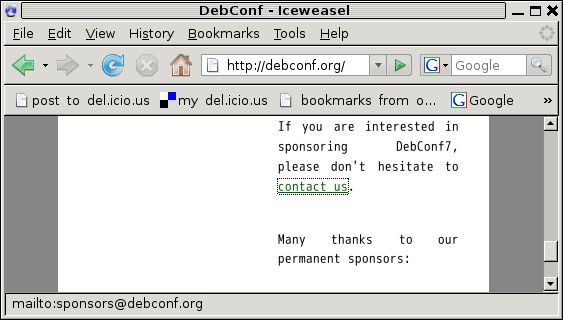
\includegraphics[width=1\hsize]{image200707/debconf-sponsor.png}

 \url{http://www.debconf.org}にアクセスすると、コンタクト先がかいてありま
す。このメールアドレスに、スポンサーしたい旨メールで表明してください。

\end{frame}


\section{サマリー}

\begin{frame}{サマリー}

\begin{tabularx}{\hsize}{|l|X|X|}
\hline
 & 要素 & 例 \\
\hline
Why & 経済的なみかえり & 
	 Debian に金を出さないと不利になる、Debconfに広告スポンサーとし
	 て金を出すことで売り上げが向上する
% 、Debianのメンバーを採用したいから
% 、企業間のつきあい
	 \\
When & Debconfの開催 & \\
How & debconf.org にメールを送信 & \\
What & 会場、ピザ、ビール
% サーバ、ネットワーク機器、ネットワーク回線、会場、Tシャツ、ノート、ペン
& \\
Who & 企業 & \\
Where &  & \\
\hline
\end{tabularx}
\end{frame}


\begin{frame}{Debconfに参加するメリット}
  \begin{tabularx}{\hsize}{|c|X|X|}
 \hline
 & 参加した場合 & 参加しなかった場合 \\
 \hline
 コード	& 合宿してコードがかける &  \\
 \hline
 文書化	& 合宿して文書がかける&  \\
 \hline
 議論 	& 直接議論できる &  \\
 \hline
 発表 	& セッションに参加して発表でき、発表をきくことができる。 &  \\
 \hline
&&\\
 \hline
&&\\
 \hline
 \end{tabularx}
\end{frame}

\begin{frame}{日本でDebconfを開催するメリット}
 
\end{frame}

\begin{frame}{Debconf を日本で開催した場合}
 
参加者の負担は?

  \begin{tabularx}{\hsize}{|c|X|X|X|}
 \hline
 & フランス & アメリカ & 南米 \\
 \hline
成田 & 828 & 809 & 1600 \\
千歳 &980 & 1197 &2121 \\
関西 &736 & 809 &1718 \\
沖縄 &1485 & 1197 &4307 \\
 \hline
 \end{tabularx}


\end{frame}


\section{最近のイベント}
\begin{frame}{最近のイベント}
\begin{itemize}
 \item 8月 夏祭り
 \item 8月 Debian 14周年
 \item 10月5-6日 OSC Tokyo/Fall
\end{itemize}
\end{frame}

\end{document}
